\part[The Java Ecosystem]{The Java Ecosystem}
\section{A History Lesson}

\begin{frame}{Once upon a time\ldots}
\visible<2->{in the land of computers there were 10101110010101101\ldots\\}
\visible<3->{then assemblers came along\ldots\\}
\visible<4->{followed by compilers\ldots\\}
\visible<5->{and they lived happily ever after\ldots \visible<6->{\alert{NOT!}}}
\end{frame}

\begin{frame}[fragile]{Portability}
\begin{block}{\alert{Platform Dependency}}
\begin{lstlisting}
for(os <- List("linux", "mac", "windows"))
  println("If you compile a C program under " + os
            + "you can run it only on " + os + ".")
\end{lstlisting}
\end{block}
\pause
Sometimes a recompilation is not sufficient. \alert{The code} has to be adapted!
\pause
\begin{block}{\textcolor{green}{Platform Independency}}
Write Once, Run Anywhere.
\end{block}
\end{frame}

\begin{frame}{Let's take a look under the hood}
\begin{center}
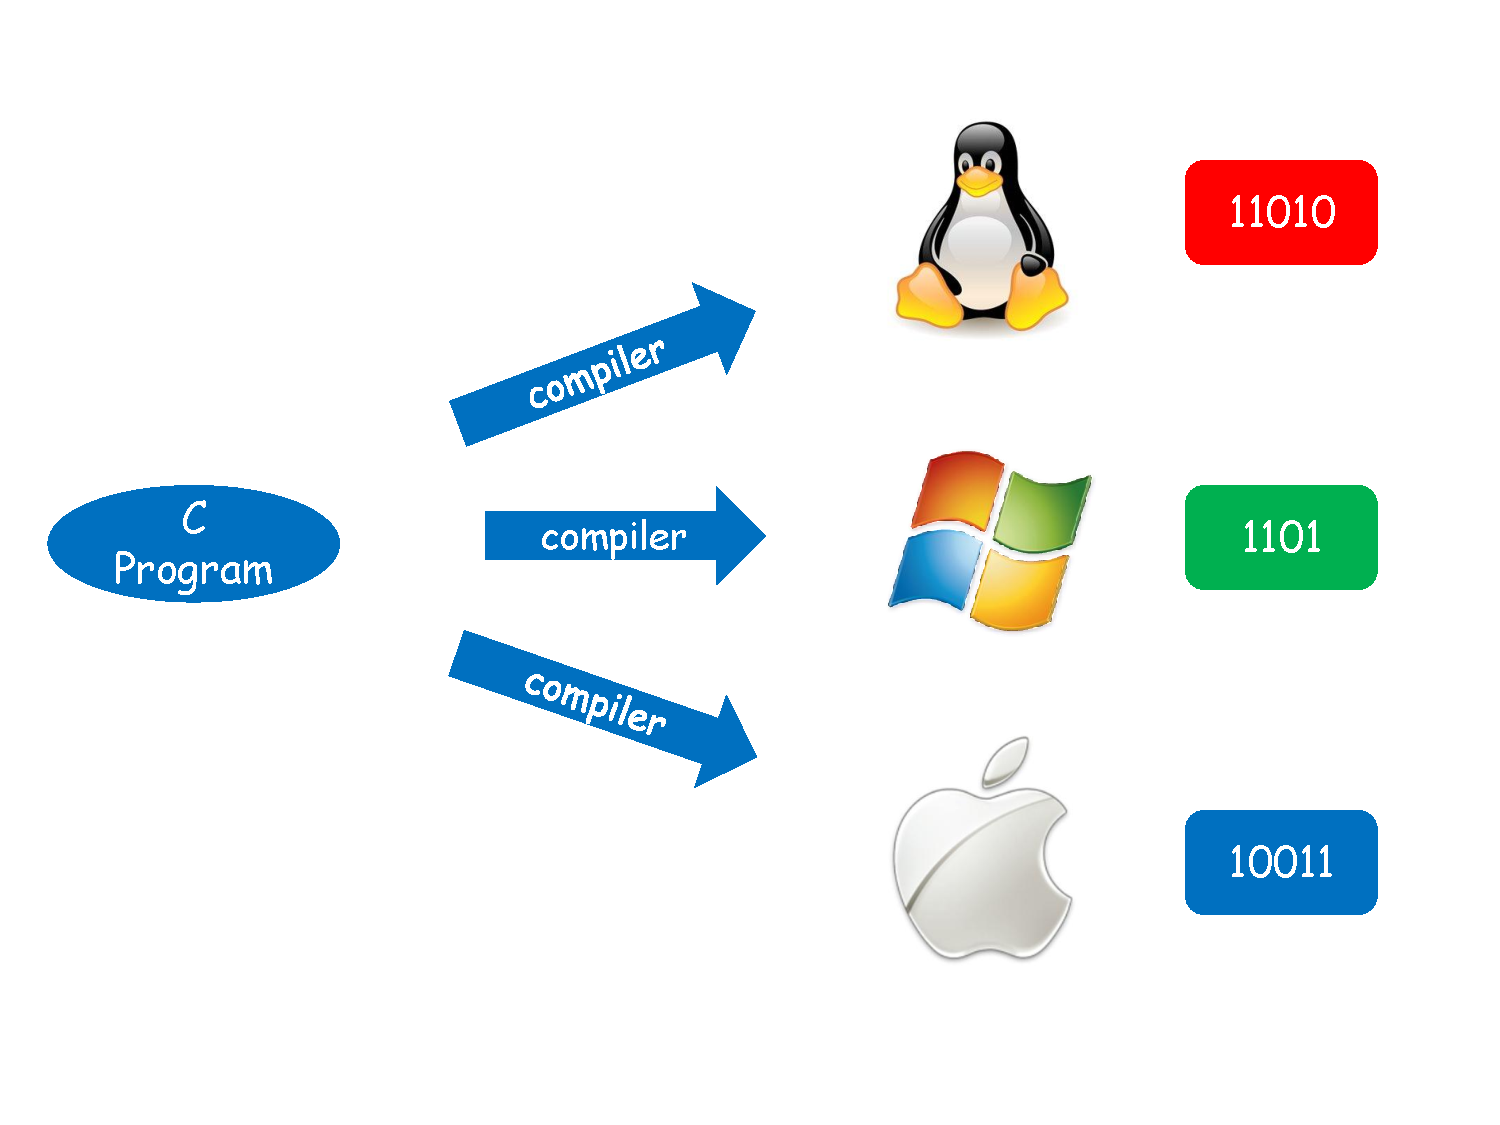
\includegraphics[scale=0.45]{resources/PlatformDependency.pdf}
\end{center}
\end{frame}

\part[Introducing Scala]{Introducing Scala}
\part[Programming Paradigms]{Programming Paradigms}
\part[Scala's Development Environment]{Scala's Development Environment}
\part[Programming Styles]{Programming Styles}
\part[Higher-Order Functions]{Higher-Order Functions}
\part[Growing The Language]{Growing The Language}
\part[TDD \& Clean Code]{Test-driven Development \& Clean Code}
\part[Pattern Matching]{Pattern Matching}
\part[Traits]{Traits}
\part[Collections]{Collections}
\part[Concurrency]{Concurrency}
\part[DSLs]{Domain Specific Languages}
\part[Higher-Kinded Types]{Higher-Kinded Types}
